% %%%%%%%%%%%%%%%%%%%%%%%%%%%%%%%%%%%%%%%%
% Beamer Presentation
% LaTeX Template
% Version 1.0 (10/11/12)
%
% This template has been downloaded from:
% http://www.LaTeXTemplates.com
%
% License:
% CC BY-NC-SA 3.0 (http://creativecommons.org/licenses/by-nc-sa/3.0/)
%
%%%%%%%%%%%%%%%%%%%%%%%%%%%%%%%%%%%%%%%%%

%----------------------------------------------------------------------------------------
%	PACKAGES AND THEMES
%----------------------------------------------------------------------------------------

\documentclass{beamer}

\usetheme{texsx}
\usepackage{graphicx} % Allows including images
\usepackage{booktabs} % Allows the use of \toprule, \midrule and \bottomrule in tables
\usepackage{url}
\usepackage{listings}

%----------------------------------------------------------------------------------------
%	TITLE PAGE
%----------------------------------------------------------------------------------------

\title[Unsupervised Representation Learning with Deep Convolutional
Generative Adversarial Networks]{Presentation on ``Unsupervised Representation 
Learning with Deep Convolutional Generative Adversarial Networks,'' by Alec Radford, Luke Metz, and Soumith Chintala} % The short title appears at the bottom of every slide, the full title is only on the title page

\author[Joh Hancock]{John Hancock \texttt{jhancoc4@fau.edu}}
\date{\today} % Date, can be changed to a custom date

\begin{document}

\begin{frame}
\titlepage % Print the title page as the first slide
\end{frame}

\begin{frame}
\frametitle{Overview} % Table of contents slide, comment this block out to remove it
\tableofcontents % Throughout your presentation, if you choose to use \section{} and \subsection{} commands, these will automatically be printed on this slide as an overview of your presentation 
\end{frame}

%----------------------------------------------------------------------------------------
%	PRESENTATION SLIDES
%----------------------------------------------------------------------------------------
\section{Introduction}
%------------------------------------------------

\begin{frame}
\frametitle{Introduction}
\framesubtitle{Caveat}
\begin{itemize}
    \item For the remainder of this presentation, we will refer to the paper
entitled , ``Unsupervised representational learning with deep convolutional
generative adversarial networks,'' as,  ``the DCGAN's paper,'' or by its
reference number \cite{repLearnDcgan}, and Alec Radford,  Luke Metz, and Soumith 
Chintala as, ``the authors.''
\end{itemize}
\end{frame}


%------------------------------------------------
\section{Background} 
% Sections can be created in order to organize your presentation into discrete blocks, all sections and subsections are automatically printed in the table of contents as an overview of the talk
%------------------------------------------------
\begin{frame}[allowframebreaks]
\frametitle{Background}
A generative adversarial network (GAN) is a neural network with two components. 
Goodfellow \textit{et. al} invent GAN's in \cite{gan}. To a first approximation,
GAN's work as follows:
\begin{itemize}
  \item The first component is a \textit{generator} that learns to transform vectors 
    of random numbers into output values that resemble instances from some dataset.  
  \item The second component is a \textit{discriminator} that classifies things into 
  two categories:
  \begin{itemize}
    \item the class of instances of the dataset, and
    \item the class of generator outputs.
  \end{itemize}
  \item ``At convergence, the generator’s samples are indistinguishable from real data,
     and the discriminator outputs $\frac{1}{2}$ everywhere. The discriminator may 
     then be discarded" \cite{deepLearnBookGenCh}. from \underline{Deep learning} , 
     Goodfellow \textit{et al.} 
\end{itemize}
\end{frame}

%------------------------------------------------
\begin{frame}[allowframebreaks]
\frametitle{Background}
\begin{itemize}

\item ... or not.  The authors of the DCGAN paper find a use for the discriminator.
  \item In the context of this paper, the outputs are images.  However, 
   researchers use GAN's where the generators create other artifacts. We find
   an extensive list on Github  \cite{ganList} of over 500 research projects. 
   Some examples from this list are:
  \begin{itemize}
    \item imputing missing values in datasets,
    \item generating music,
    \item fraud detection, and
    \item playing chess.
  \end{itemize}
\end{itemize}
\end{frame}

%------------------------------------------------

\section{Contributions}
\begin{frame}[allowframebreaks]
\frametitle{Contributions}

The authors of the paper make several contributions they...
\begin{itemize}
  \item invent an architecture for DCGAN's,
  \item use the convolutional layer filters of trained DCGAN's discriminators as 
    feature extractors for doing classifications,
  \item demonstrate that after training the DCGAN, its filters learn how to
    represent images, and
  \item present a method of doing vector arithmetic using DCGAN inputs to do 
    inferences \emph{{\`a} la} Word2Vec \cite{word2Vec}.
\end{itemize}
\end{frame}

%------------------------------------------------
\section{Architecture}

\begin{frame}[allowframebreaks]
\frametitle{Architecture Diagram}


\tikzstyle{format} = [draw, thin, fill=blue!50!cyan!80]
\tikzstyle{medium} = [draw, thin, fill=red!40]
\tikzstyle{cost} = [draw, thin, fill=green!20]
\tikzstyle{input} = [draw, thin, fill=brown!10]
\tikzstyle{operator} = [circle, draw, thin, fill=green!20]

\begin{footnotesize}
\begin{figure}
\begin{tikzpicture}[thick]

\node[input] (noise) at (0,0) {Noise Vector};

\node[input] (dataset) at (0,2) {Dataset};

\node[format](generator) at (3,0) {Generator G};

\node[medium] (gOptimizer) at (6.25, 0) {Optimizer};

\node[format](discriminator) at (3,2) {Discriminator D};

\node[medium] (dOptimizer) at (3,4) {Optimizer};

\node[cost] (dCostDataset) at (6.25,3){D Cost Dataset};

\node[cost] (dCostGenerated) at (6.25,2){D Cost Generated};

\node[cost] (gCostGenerated) at (6.25,1){G Cost Generated};

\node[operator] (adder) at (5.5,4){+};

\draw[->] (noise) -- (generator);

\draw[->] (generator) -- (discriminator) ;

\draw[->] (gOptimizer) -- (generator);

\draw[->] (gCostGenerated) -- (gOptimizer);

\draw[->] (dataset) -- (discriminator);

\draw[->] (discriminator) -- (4.5, 2) |- (dCostDataset);
\draw[->] (discriminator) -- (4.5,2) |- (gCostGenerated);
\draw[->] (discriminator) -- (dCostGenerated);

\draw[->] (dCostGenerated) -- (8,2) |- (adder);
\draw[->] (dCostDataset) -- (8,3) |- (adder);

\draw[->] (adder) -- (dOptimizer);

\draw[->] (dOptimizer) -- (discriminator);

\end{tikzpicture}
\end{figure}
\end{footnotesize}
\end{frame}

%------------------------------------------------

\begin{frame}[allowframebreaks]
\frametitle{Architecture}
\framesubtitle{Generator Diagram from Paper \cite{repLearnDcgan}}
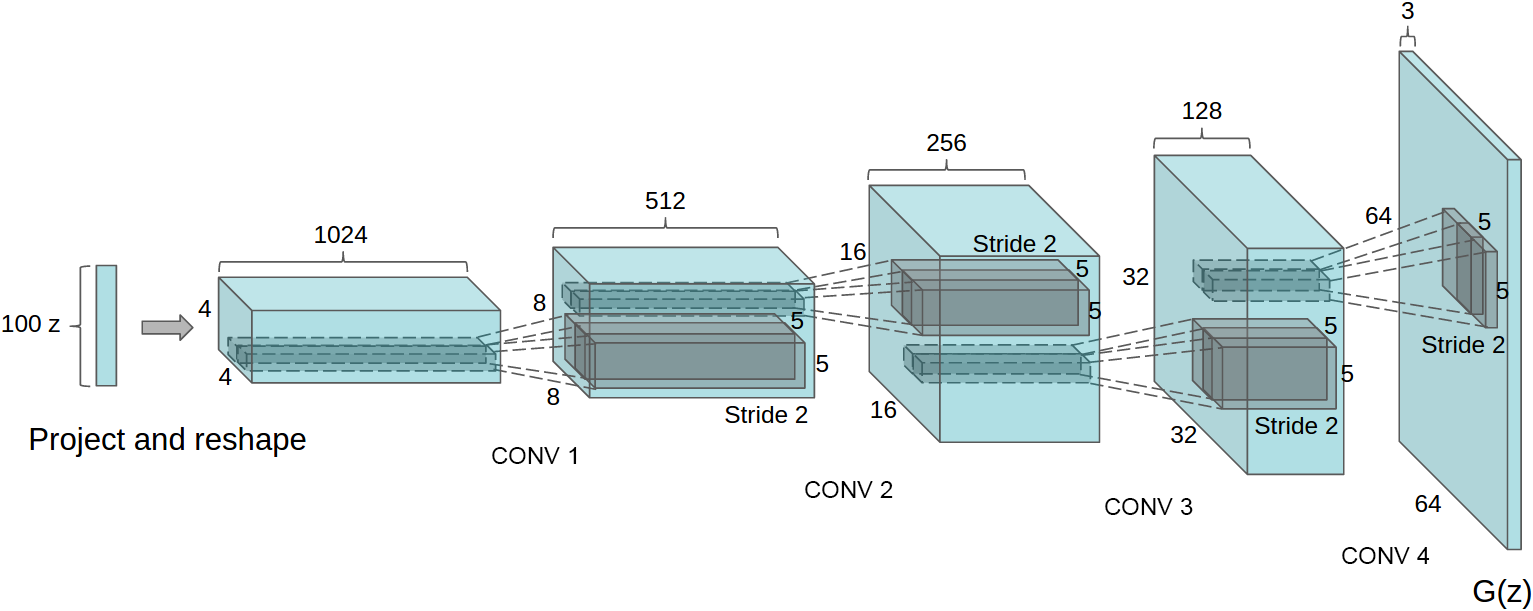
\includegraphics[scale=0.2]{generator-diagram}
\end{frame}
%------------------------------------------------

%------------------------------------------------

\begin{frame}[allowframebreaks]
\frametitle{Results}
\begin{itemize}
  \item The authors use three datasets for training:
  \begin{itemize}
    \item Large Scale Scene Understanding (LSUN),
    \item Imagenet 1-K, and
    \item Faces.
  \end{itemize}  
  \item The authors two datasets for evaluating unsupervised learning: Canadian 
    Institute for Advanced Research (CIFAR) 10 StreetView House Numbers (SVHN)
\end{itemize}
\end{frame}

%------------------------------------------------

\begin{frame}[allowframebreaks]
\frametitle{Results - LSUN}
\framesubtitle{LSUN - Generator representation learning}
\begin{itemize}
  \item The authors use images of bedrooms from the LSUN dataset
  \cite{lsunDataset} as input to their DCGAN.

  \item Then they find a way to identify and remove the generators feature maps
  \cite{repLearnDcgan} associated with windows.  Note: see explanation of feature
  maps in Dr. Zhu's lectures on CNN's \cite{cnnlecture}. 

  \item After removing these feature maps, the generator no longer produces images
    of bedrooms with windows.

  \item The authors claim that this experiment proves the generator is learning
   representations of objects in an unsupervised manner. 
\end{itemize}
\end{frame}

%------------------------------------------------

\section{Results}
\begin{frame}[allowframebreaks]
\frametitle{Results - LSUN}
\framesubtitle{Discriminator -  Representation learning visualization}
\begin{itemize}
\item The authors did some processing known as guided backpropagation on the
first 6 convolutional features of the last convolutional layer of their DCGAN's
discriminator to create the image below.  

\item This is proof that the discriminator  is learning features.  
  \begin{itemize} 
  \item Note on the
  left-hand side taken before training that the pictures look like entire bedrooms,
  but after training the pictures have key portions of a bedroom scene, like windows
  and beds.
  \item This demonstrates how the DCGAN is learning to represent objects in
  images.
  \end{itemize}
\end{itemize}
\begin{figure}
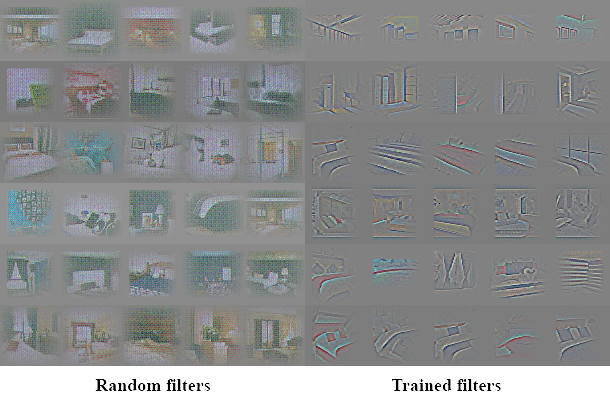
\includegraphics[scale=0.35] {feature-maps}
\caption{This image is coped from the paper \cite{repLearnDcgan}.}
\end{figure}
\end{frame}


%------------------------------------------------

\begin{frame}[allowframebreaks]
\frametitle{Results - CIFAR}
\begin{itemize}
 \item The authors use images from the \textbf{\textit{Imagenet 1-k}} dataset as input to a DCGAN.
 \item After training, they take all the convolutional layers the discriminator
 learns, and use them as feature extractors. 
 
\item However they accomplished this, the authors then use the feature extractor 
  they created from the DCGAN's discriminator for a support vector machine based
  classifier.
\item They then used images from \textbf{\textit{CIFAR-10}} dataset as inputs to this
  classifier that they report as 82.8\% accurate. They mention similar K-Means based
  approaches that get lower accuracy so the result is competitive and noteworthy.
 
\item This result is remarkable because they built a classifier that is able to
  correctly categorize images from one dataset, based on unsupervised learning
  methods involving a different dataset.  It proves GAN's have generalization power.


\end{itemize}
\end{frame}

%------------------------------------------------

\begin{frame}[allowframebreaks]
\frametitle{Results - SVHN}
\begin{itemize}
 \item We interpret the wording the authors use in section 5.2 to mean that the
   authors use images from the SVHN dataset as input to a DCGAN.
 \item It is not clear what the authors mean by, ``non-extra set'' they use 
  for training their model.
 \item Is is our understanding that they train a DCGAN on the SVHN dataset, and
  then build a feature extractor similar to what they do with the DCGAN they
  build for Imagenet 1-k.
\item Using this feature extractor, the authors then incorporate this into an
  L2-SVM classifier that we suppose is classifying images from SVHN.
\item The notable result the authors report is that the classifier they build in
  this manner gets a lower error rate than a similar classifier built with a
  standard convolutional neural network.

\end{itemize}
\end{frame}

%------------------------------------------------

\begin{frame}[allowframebreaks]
\frametitle{Results - Faces}
\begin{itemize}
\item The authors write that they create a faces dataset of images of faces from
  randomly selected web sites.

\item After training the DCGAN on this dataset the authors do arithmetic on
what they call, the ``Z-vectors of sets of exemplar samples for visual concepts.''

\begin{itemize}
  \item We take this to mean they were able to find groups of vectors of random
  numbers they used for inputs to the generator that produce images that look like
  something in particular, for example: a smiling man.

  \item An important clue for our understanding of the term Z-vector is that the
  first input parameter of the generator function in the code that accompanies this
  paper \cite{dcganCode} is named, ``Z,'' and other vectors involving random numbers
  in the code also start with the letter, `z.'
  \end{itemize}

\end{itemize}
\end{frame}

%------------------------------------------------

\begin{frame}[allowframebreaks]
\frametitle{Results - Faces}
\begin{itemize}
\item The authors then do vector addition and subtraction with vectors they obtain
from the average values of vectors in different exemplar sets.

\item The authors then use the vectors are the results of these arithmetic operations
as inputs to the generator.

\item Please see the amazing result on the next slide. We feel this is the strongest
result of the paper. 
\end{itemize}
\end{frame}

%------------------------------------------------

\begin{frame}[allowframebreaks]
\frametitle{Results - Faces}
\framesubtitle{This image is from the DCGAN paper \cite{repLearnDcgan}:}
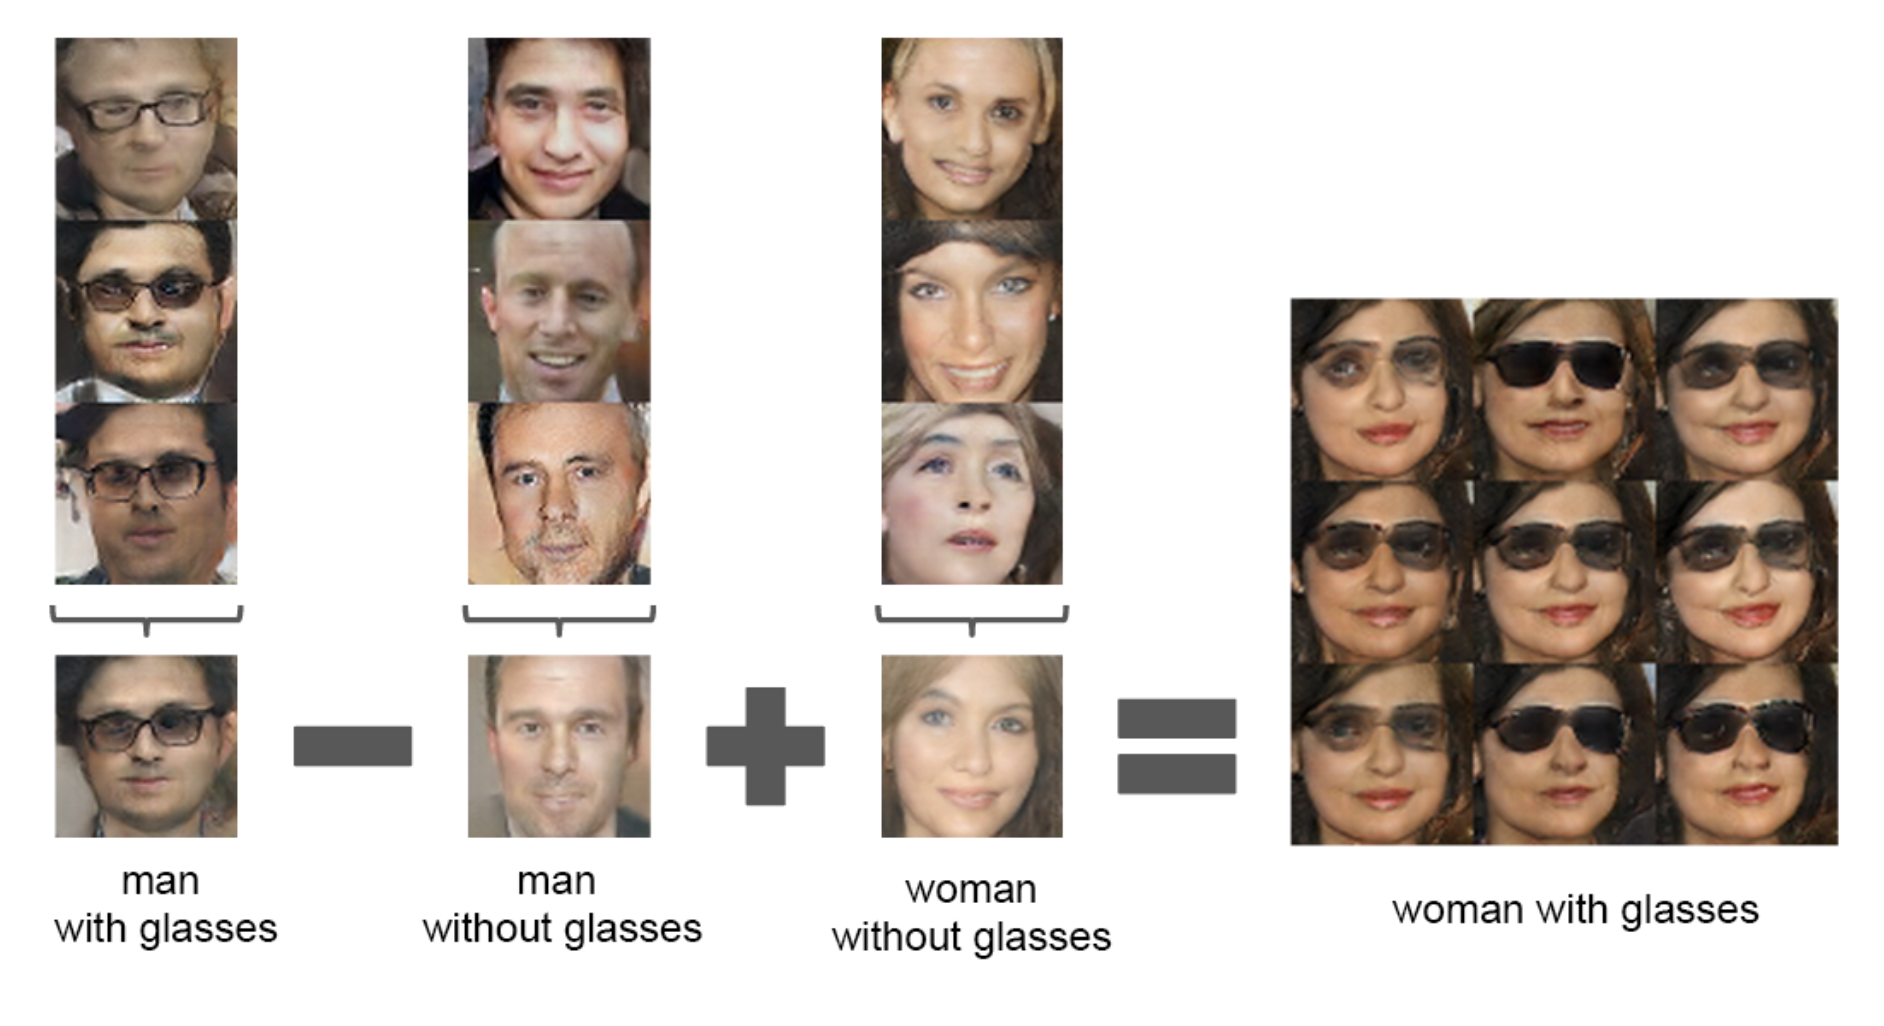
\includegraphics[scale=0.25]{woman-with-glasses}
\end{frame}

%------------------------------------------------

\section{Conclusions}
\begin{frame}[allowframebreaks]
\frametitle{Conclusions}
\begin{itemize}
\item The authors present a working architecture for GAN's that uses
convolutional, and fractionally-strided (also known as deconvolutional) neural
networks.
\item Authors show how the convolutional and fractionally-strided convolutional  
layers indicate their DCGAN is automatically learning representations in an 
unsupervised manner.
\item The source code that the authors wrote is publicly available and it
bolsters their claims; one can access the source code on Github
\cite{dcganCode}, or a derivative work such as \cite{dcganTf} and confirm
that it generates outputs as advertised.
\end{itemize}
\end{frame}

%------------------------------------------------
% https://ieee-dataport.org/sites/default/files/analysis/27/IEEE%20Citation%20Guidelines.pdf

\begin{frame}[allowframebreaks]
\frametitle{References}
\footnotesize{
\begin{thebibliography}{99} % Beamer does not support BibTeX so references must be inserted manually as below

\bibitem{repLearnDcgan} S. Chintala, L. Metz, and A. Radford, 
Unsupervised representation learning with deep convolutional generative 
adversarial networks.  2016. [Online]. Available: arXiv:1511.06434v2 [cs.LG]

\bibitem{dcganCode} S. Chintala, L. Metz, and A. Radford, dcgan\_code. (2016,
May).  Available: \url{https://github.com/Newmu/dcgan\_code}. [Accessed Nov. 19,
2018].

\bibitem{lsunDataset} Large Scale Scene Understanding Challenge (2017, July).
Available: \url{http://lsun.cs.princeton.edu/2017/}. [Accessed Nov. 19, 2018].

\bibitem{dcganTf} T Kim. (2018, August).  Available: \url{https://github.com/carpedm20/DCGAN-tensorflow}. [Accessed Nov. 19, 2018].


\bibitem{gan} Y. Bengio, A. Courville,I. Goodfellow, M. Mirza, S. Ozair,  
J. Pouget-Abadie,  D. Warde-Farley, B. Xu, Generative adversarial nets. 2014. 
[Online]. Available: arXiv:1406.2661v1 [stat.ML]

\bibitem{word2Vec} T. Mikolov, I. Sutskever, K. Chen, G. Corrado, J. Dean,
``Distributed Representations of Words and Phrases and their Compositionality,''
Advances in Neural Information Processing Systems 26 (NIPS 2013), 2013. 
[Online] Available: \url{http://papers.nips.cc/paper/5021-distributed-}representations-of-words-and-phrases-and-their-compositionality.pdf

\bibitem{slidetemplate} Creodocs Limited,``Beamer Presentation,''
\emph{latextemplates.com}, 2018. [Online], Available: 
\url{http://www.latextemplates.com/templates/presentations/1/presentation\_1.zip}. [Accessed Nov. 10, 2018].

\bibitem{ieeeStyle} IEEE, Piscataway, NJ, USA. \emph{IEEE Editorial Style Manual}. 2016.
[Online]. Available: \url{http://ieeeauthorcenter.ieee.org/wp-content/uploads/IEEE\_Style_Manual.pdf}, [Accessed Nov. 11, 2018].

\bibitem{deepLearnR} F. Chollet, and J.J. Allaire.  
\textit{Deep Learning with R}. Manning Publications 2018. [E-Book] Available: Safari
E-Book.

\bibitem{deepLearnBookGenCh} Y. Bengio, A. Courville, I. Goodfellow. (2016).
``Chapter 20 Deep Generative Models,'' 2016. [Online] Available:
\url{https://www.deeplearningbook.org/contents/generative\_models.html}.
[Accessed: Nov. 20, 2018].

\bibitem{ganList} A. Hindupur, ``A list of all named GANs!'' github.com, Sep. 30,
2018. [Online]. Available: \url{https://github.com/hindupuravinash/the-gan-zoo}. 
[Accessed Nov. 21, 2018]. 

\bibitem{cnnlecture} Xingquan Zhu. 2018. Convolutional Neural Networks (CNN) retrieved
 October 22, 2018 from \url{https://canvas.fau.edu/files/14310707/download?download\_fr
d=1}

\end{thebibliography}
}
\end{frame}

%------------------------------------------------

\begin{frame}
\Huge{\centerline{The End}}
\end{frame}

%----------------------------------------------------------------------------------------

\end{document} 
